%Schriftgr"osse, Layout, Papierformat, Gleichungen Linksb"undig
\documentclass[10pt,twoside,a4paper,fleqn]{article}
\usepackage[left=1cm,right=1cm,top=1cm,bottom=1cm,includeheadfoot]{geometry}
\usepackage[utf8]{inputenc}
\usepackage[ngerman]{babel,varioref}%ngerman
%Packages - Von LinAlg Formelsammlung kopiert! "Uberpr"ufen ob die alle notwendig sind
\usepackage{amsmath,amssymb,fancybox,graphicx,color,lastpage,wrapfig,fancyhdr,hyperref,verbatim}
\usepackage{listings}
%Package f"ur Bilder im Fliesstext
\usepackage{multicol}

%Package f"ur Tabelle im Querformat
\usepackage{rotating}

%Paragraphe ebenfalls nummerieren
\setcounter{secnumdepth}{4}

\raggedright
%Titel, Autor
\title{Digitaltechnik Zusammenfassung}
\author{Giachen Koeeppel, Damian Koeppel}

%Seitenstyle
\pagestyle{fancy}
\lfoot{{Giachen und Giari K\"oppel, C. Gwerder, S.K\"orner}}



%Document Anfang
\begin{document}

\begin{multicols}{2}
\section{Digital vs. Analog}
Digital ist st"orsicher, hat keine St"orfortpflanzung und erlaubt einfachen Entwurf und Test mit Hilfe von CAD.

Analog ist st"oranf"allig, komplex, erfordert Spezialisten, Entwurf weitgehend von Hand, etc.

Digital ist aber langsamer, da alles in der Welt analog ist. F"ur Digital brauchts also noch eine Umwandlung.
\subsection{AD-Wandlung}
$$ \text{Abstastfrequenz} \geq 2\cdot f_{max}$$\\
$$ \Delta \text{Quantisierungsstufe} = 2 \cdot \text{Quantisierungsfehler}$$\\
$$\text{Amplitudenauflösung: Dynamik; SNR} \approx 6dB/bit$$
\end{multicols}

\begin{multicols}{2}
\section{Digital}
\subsection{FETs (selbstsperrend)}
	\begin{tabular}{|l|c|p{2.2cm}|p{2cm}|}
		\hline
		 & & $U_{GS}$ (leitend) & $I_D$ bei $U_{DS}$\\
		\hline
		n-FET & \raisebox{-.8\totalheight}{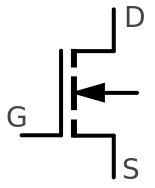
\includegraphics[width=0.05\textwidth]{pics/nFET}} & positiv & positiv \\
		\hline
		p-FET & \raisebox{-.8\totalheight} {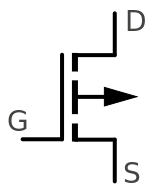
\includegraphics[width=0.05\textwidth]{pics/pFET}} & negativ & negativ \\
		\hline
	\end{tabular}
$$\hspace{-1.5cm}\text{Gatteräquivalent } n_{ge} = \frac{n_{trans}}{4}$$\\

\subsection{Zahlensysteme}
\subsubsection{Binär}
\paragraph{Bereichsüberschreitung Zweierkomplement}
\begin{itemize}
	\item [] Richtig $\Rightarrow Carry_n = Carry_{n-1}$\\
		  Falsch $\Rightarrow Carry_n \neq Carry_{n-1}$\\
\end{itemize}

\paragraph{Umwandeln von Komastellen}
\begin{itemize}
	\item [] $Komastelle_0 \cdot Basis = Ganzzahl_1,Komastelle_1$\\
		     $\dots$Weiterführen bis Genauigkeit erreicht ist\\		     
                     $Komastelle_{n-1} \cdot Basis = Ganzzahl_{n}, Komastelle_{n}$\\
			
	\item [] Wert hinter Koma in neuem Zahlensystem $= Ganzzahl_{1}\cdot Basis^{-1} + \dots+ Ganzzahl_n\cdot Basis^{-n}$\\
		Somit werden Stellen hinter Komma von oben nach unten aufgeschrieben

	\item [] \textbf{Beispiel} mit Zahl 2.7$_{10}$\\
		$\left.\begin{array}{ccc}
			2 / 2 & = 1 & R 0\\
			1 / 2 & = 0 & R 1
		\end{array}\right\uparrow$\\
		$\left.\begin{array}{cccl}
			0.7 \cdot 2 &= &\mathbf{1}.4\\
			0.4 \cdot 2 &= &\mathbf{0}.8\\
			0.8 \cdot 2 &= & \mathbf{1}.6\\
			0.6 \cdot 2 &= & \mathbf{1}.2\\
		\end{array}\right\downarrow$\\
		
		Zahl = 10,\textbf{1011}$\dots_2$ \\
	\end{itemize}
\end{multicols}
\vspace{-20pt}

%\section{Schaltalgebra}
\subsection{Rechenregeln}

\textbf{Allg. $\Rightarrow$ Punkt vor Strich oder $\land$ vor $\lor$}

	\begin{tabular}{llll}
		Verkn"upfung mit 0 & $ a \lor 0 = a $ & $ a \land 0 = 0 $ & $ a \not= 0 = a $\\
		Verkn"upfung mit 1 & $ a \lor 1 = 1 $ & $ a \land 1 = a $ & $ a \not= 1 = \overline{a} $ \\
		Verkn. mit sich selbst & $ a \lor a = a $ & $ a \land a = a $ & $ a \not= a = 0 $ \\
		Verkn. mit Inversem & $ a \lor \overline{a} = 1 $ & $ a \land \overline{a} = 0 $ & $ a \not= \overline{a} = 1 $ \\
		\\
		Kommutativgesetz & $ a \lor b = b \lor a $ & $ a \land b = b \land a $ & $ a \not= b = b \not= a $\\
		Assioziativgesetz & $ (a \lor b) \lor c = a \lor (b \lor c) $ & $ (a \land b) \land c = a \land (b \land c) $ & $ (a \not= b) \not= c = a \not= (b \not= c) $ \\
		Distributivgesetz & $ a \land (b \lor c) = (a \land b) \lor (a \land c) $ & $ a \lor (b \land c) = (a \lor b) \land (a \lor c) $ & $ a \land (b \not= c) = (a \land b) \not= (a \land c) $ \\	
		\end{tabular}
\subsection{Vereinfachungen}
\begin{tabular}{lllll}
	$ a \lor (a \land b) = a $ & $(a \land b) \lor (a \land \overline{b}) = a $ &\hspace{2.0cm} &
	$  (a \land\overline{b}) \lor b = a \lor b$ & $ (a \land \overline{b}) \not= b = a \lor b $\\
	$  a \land (a \lor b) = a $ & $ (a \lor b) \land (a \lor \overline{b}) = a $ &\hspace{2.0cm}&
	$ (a \lor \overline{b}) \land b = a \land b $ &$(a \not= \overline{b}) \land b = a \land b  $\\
\end{tabular}

\subsection{Shannon und DeMorgan}
\begin{multicols}{2}
	\textbf{DeMorgan}\\
	$a \land b = \overline{\overline{(a \land b)}}= \overline{(\overline{a} \lor \overline{b})}$\\
	$a \lor b = \overline{\overline{(a \lor b)}} = \overline{(\overline{a} \land \overline{b})}$

	\textbf{Shanon} (Vereinfachter Demorgan)\\
	- alle Variablen negieren\\
	- alle Operatoren negieren ($\lor \rightarrow \land / \land \rightarrow \lor$)\\
	- ganzer Ausdruck negieren
\end{multicols}
\begin{tabular}{lll}
	Ursprungsschaltung: & Shannon & DeMorgan\\
		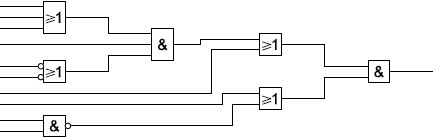
\includegraphics[width=0.3\textwidth]{pics/shanonursprung} & 
		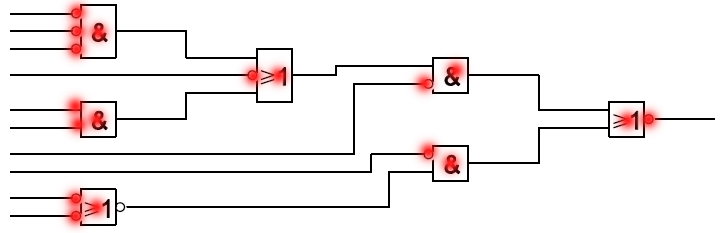
\includegraphics[width=0.3\textwidth]{pics/shanonende} &
		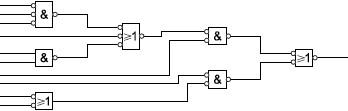
\includegraphics[width=0.3\textwidth]{pics/demorganende}\\
\end{tabular}


\subsection{Wahrheitstabelle, KDNF, KKNF}
\begin{multicols}{2}
\subsubsection{KDNF (Kanonisch  Disjunktive Normalform)}
\vspace{-5pt}
\textbf{Minterm}$~~$ \\
Zeile in WHT mit Funktionswert = \textbf{1}\\
$\rightarrow$ Eingangsvariablen AND($\land$)-Verknüpfen \\
$\rightarrow $ Eingangsvariable mit Wert \textbf{0} invertieren\\
\textbf{DNF (Sums of products)}\\
Minterme OR($\lor$)-Verknüpfen\\
\textbf{Kurzschreibweise:}\\
DNF: $ b = \lor([1],[3],5) $ \\
Zahl entspricht Zeile, Eckige Klammern bedeutet don't care.\\ 

\subsubsection{KKNF (Kanonisch Konjunktive Normalform)}
\vspace{-5pt}
\textbf{Maxterm}$~~$ \\
Zeile in WHT mit Funktionswert = \textbf{0}\\
$\rightarrow$ Eingangsvariablen OR($\lor$)-Verknüpfen \\
$\rightarrow $ Eingangsvariable mit Wert \textbf{1} invertieren\\
\textbf{KNF (Products of sums)}\\
Maxterme AND($\land$)-Verknüpfen\\
\textbf{Kurzschreibweise:}\\
KNF: $ a = \land([1],[2],3) $ \\
Zahl entspricht Zeile, Eckige Klammern bedeutet don't care.\\ 

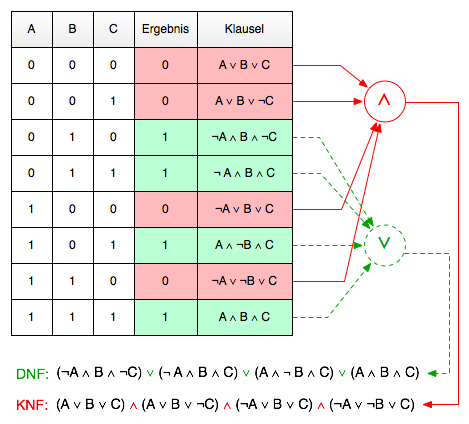
\includegraphics[width=0.5\textwidth]{pics/KNFDNF}
\end{multicols}

\subsection{Karnaugh-Diagramm}
\begin{tabular}{lll}
	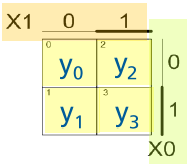
\includegraphics[width=0.1\textwidth]{pics/kv/2erKV} & 
	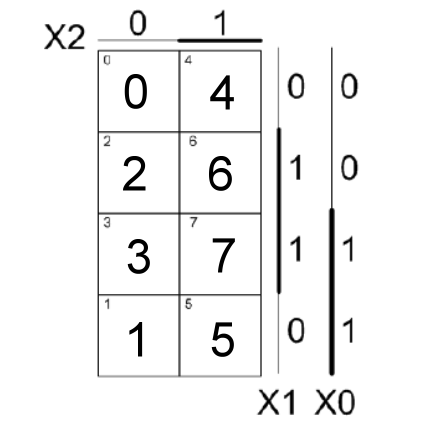
\includegraphics[width=0.1\textwidth]{pics/kv/3erKV} &
	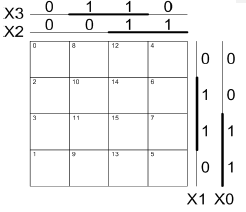
\includegraphics[width=0.15\textwidth]{pics/kv/4erKV}\\
\end{tabular}
\subsection{Arbeiten mit KV-Diagramm}
\begin{enumerate}
\setlength{\itemsep}{1pt}
  \setlength{\parskip}{0pt}
  \setlength{\parsep}{0pt}
\item Aufstellen der Wahrheitstabelle\\
\item "Ubertragen der Funktionswerte der Wahrheitstabelle in KV Diagramm\\
\item M"oglichst grosse Gruppen à $2^n$ Felder bilden\\
\begin{tabular}{|p{7cm}|p{7cm}}
	\textbf{DNF} & \textbf{KNF} \\
	Gruppen von Feldern mit Wert 1 oder d & Gruppen von Feldern mit Wert 0 oder d\\
\end{tabular}
\item Terme aus KV-Diagramm lesen\\
\begin{tabular}{|p{7cm}|p{7cm}}
	Variablen in Gruppe \textbf{AND}-Verknnüpfen & Variablen in Gruppe \textbf{OR}-Verknüpfen\\
	$\rightarrow$ \textbf{Variable = 0 invertieren}&$\rightarrow$ \textbf{Variable = 1 invertieren}\\
	\textbf{OR}-Verknüpfen aller Primimplikanten & \textbf{AND}-Verknüpfen aller Primimplikanten\\
\end{tabular}
\end{enumerate} % Schaltalgebra mit Logik Symbolen (V,...)
\section{Schaltalgebra}
\subsection{Rechenregeln}

\textbf{Allg. $\Rightarrow$ Punkt vor Strich oder $\cdot$ vor $+$}

	\begin{tabular}{llll}
		Verkn"upfung mit 0 & $ a + 0 = a $ & $ a \cdot 0 = 0 $ & $ a \oplus 0 = a $\\
		Verkn"upfung mit 1 & $ a + 1 = 1 $ & $ a \cdot 1 = a $ & $ a \oplus 1 = \overline{a} $ \\
		Verkn. mit sich selbst & $ a + a = a $ & $ a \cdot a = a $ & $ a \oplus a = 0 $ \\
		Verkn. mit Inversem & $ a + \overline{a} = 1 $ & $ a \cdot \overline{a} = 0 $ & $ a \oplus \overline{a} = 1 $ \\
		\\
		Kommutativgesetz & $ a + b = b + a $ & $ a \cdot b = b \cdot a $ & $ a \oplus b = b \oplus a $\\
		Assioziativgesetz & $ (a + b) + c = a + (b + c) $ & $ (a \cdot b) \cdot c = a \cdot (b \cdot c) $ & $ (a \oplus b) \oplus c = a \oplus (b \oplus c) $ \\
		Distributivgesetz & $ a \cdot (b + c) = (a \cdot b) + (a \cdot c) $ & $ a + (b \cdot c) = (a + b) \cdot (a + c) $ & $ a \cdot (b \oplus c) = (a \cdot b) \oplus (a \cdot c) $ \\	
		\end{tabular}
\subsection{Vereinfachungen}
\begin{tabular}{lllll}
	$ a + (a \cdot b) = a $ & $(a \cdot b) + (a \cdot \overline{b}) = a $ &\hspace{2.0cm} &
	$  (a \cdot\overline{b}) + b = a + b$ & $ (a \cdot \overline{b}) \oplus b = a + b $\\
	$  a \cdot (a + b) = a $ & $ (a + b) \cdot (a + \overline{b}) = a $ &\hspace{2.0cm}&
	$ (a + \overline{b}) \cdot b = a \cdot b $ &$(a \oplus \overline{b}) \cdot b = a \cdot b  $\\
\end{tabular}

\subsection{Shannon und DeMorgan}
\begin{multicols}{2}
	\textbf{DeMorgan}\\
	$a \cdot b = \overline{\overline{(a \cdot b)}}= \overline{(\overline{a} + \overline{b})}$\\
	$a + b =  \overline{\overline{(a + b)}}= \overline{(\overline{a} \cdot \overline{b})}$

	\textbf{Shanon} (Vereinfachter Demorgan)\\
	- alle Variablen negieren\\
	- alle Operatoren negieren ($+ \rightarrow \cdot / \cdot \rightarrow +$)\\
	- ganzer Ausdruck negieren
\end{multicols}
\begin{tabular}{lll}
	Ursprungsschaltung: & Shannon & DeMorgan\\
		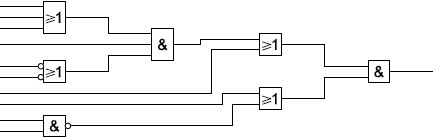
\includegraphics[width=0.3\textwidth]{pics/shanonursprung} & 
		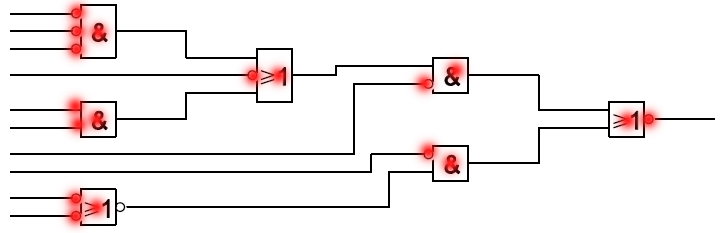
\includegraphics[width=0.3\textwidth]{pics/shanonende} &
		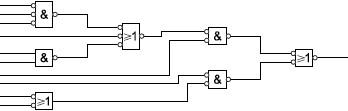
\includegraphics[width=0.3\textwidth]{pics/demorganende}\\
\end{tabular}


\subsection{Wahrheitstabelle, KDNF, KKNF}
\begin{multicols}{2}
\subsubsection{KDNF (Kanonisch  Disjunktive Normalform)}
\vspace{-5pt}
\textbf{Minterm}$~~$ \\
Zeile in WHT mit Funktionswert = \textbf{1}\\
$\rightarrow$ Eingangsvariablen AND($\cdot$)-Verknüpfen \\
$\rightarrow $ Eingangsvariable mit Wert \textbf{0} invertieren\\
\textbf{DNF (Sums of products)}\\
Minterme OR($+$)-Verknüpfen\\
\textbf{Kurzschreibweise:}\\
DNF: $ b = \#([1],[3],5) $ \\
Zahl entspricht Zeile, Eckige Klammern bedeutet don't care.\\ 

\subsubsection{KKNF (Kanonisch Konjunktive Normalform)}
\vspace{-5pt}
\textbf{Maxterm}$~~$ \\
Zeile in WHT mit Funktionswert = \textbf{0}\\
$\rightarrow$ Eingangsvariablen OR($+$)-Verknüpfen \\
$\rightarrow $ Eingangsvariable mit Wert \textbf{1} invertieren\\
\textbf{KNF (Products of sums)}\\
Maxterme AND($\cdot$)-Verknüpfen\\
\textbf{Kurzschreibweise:}\\
KNF: $ a = \&([1],[2],3) $ \\
Zahl entspricht Zeile, Eckige Klammern bedeutet don't care.\\ 

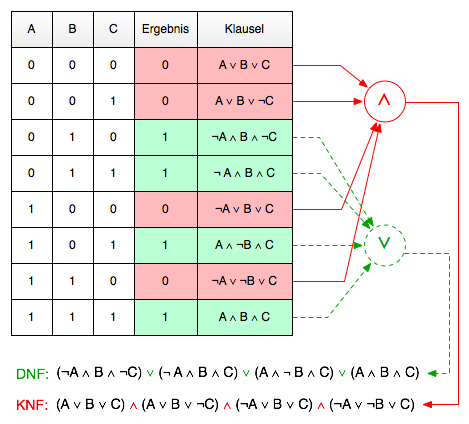
\includegraphics[width=0.5\textwidth]{pics/KNFDNF}
\end{multicols}

\subsection{Karnaugh-Diagramm}
\begin{tabular}{lll}
	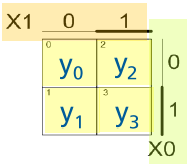
\includegraphics[width=0.1\textwidth]{pics/kv/2erKV} & 
	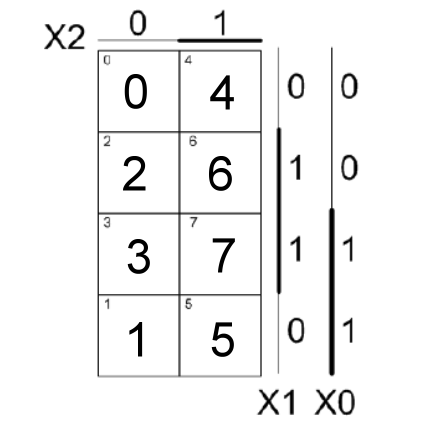
\includegraphics[width=0.1\textwidth]{pics/kv/3erKV} &
	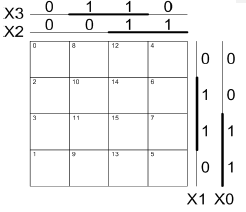
\includegraphics[width=0.15\textwidth]{pics/kv/4erKV}\\
\end{tabular}
\subsection{Arbeiten mit KV-Diagramm}
\begin{enumerate}
\setlength{\itemsep}{1pt}
  \setlength{\parskip}{0pt}
  \setlength{\parsep}{0pt}
\item Aufstellen der Wahrheitstabelle\\
\item "Ubertragen der Funktionswerte der Wahrheitstabelle in KV Diagramm\\
\item M"oglichst grosse Gruppen à $2^n$ Felder bilden\\
\begin{tabular}{|p{7cm}|p{7cm}}
	\textbf{DNF} & \textbf{KNF} \\
	Gruppen von Feldern mit Wert 1 oder d & Gruppen von Feldern mit Wert 0 oder d\\
\end{tabular}
\item Terme aus KV-Diagramm lesen\\
\begin{tabular}{|p{7cm}|p{7cm}}
	Variablen in Gruppe \textbf{AND}-Verknnüpfen & Variablen in Gruppe \textbf{OR}-Verknüpfen\\
	$\rightarrow$ \textbf{Variable = 0 invertieren}&$\rightarrow$ \textbf{Variable = 1 invertieren}\\
	\textbf{OR}-Verknüpfen aller Primimplikanten & \textbf{AND}-Verknüpfen aller Primimplikanten\\
\end{tabular}
\end{enumerate} %Schaltalgebra mit Mathematischen Symbolen (+,...)
%\section{VHDL}
	Die vollst�ndige Beschreibung des Designs besteht aus:\\
	\begin{itemize}
	\setlength{\itemsep}{1pt}
  \setlength{\parskip}{0pt}
  \setlength{\parsep}{0pt}
		\item Bibliothekenbeschreibung
		\item Schnittstellenbeschreibung
		\item Architekturbeschreibung
	\end{itemize}
	\subsection{Key Concepts}
		\begin{tabular}{ll}
			Key Concept I: & Schaltungshierarchie und Verbindung von Sub-Bl�cken (hierarchy and connectivity).\\
			Key Concept II: & Nebenl�ufige (concurrent) Prozesse und Prozess-Interaktion.\\
			Key Concept III: & Modellierung des elektrischen Verhaltens von Signalen.\\
			Key Concept IV: & Event-Based time: Simulationsmodell, das auf Events und nicht auf kontinuierlicher Zeit beruht.\\
			Key Concept V: & Parametrisierung von Modellen.
		\end{tabular}
	\subsection{Bibliotheken}
		\begin{tabular}{ll}
			work & Default-Bibliothek des Benutzers\\
			std & Enth�lt standard (Vordefinierte Datentypen und Funktionen und\\
			& textio (Dateioperationen)\\
			ieee & std\_logic\_1164: Datentypen f�r mehrwertiges Logiksystem
		\end{tabular}
		\lstinputlisting[language=VHDL,tabsize=2]{code/header.vhd}
	\subsection{Schnittstellenbeschreibung (Entity)}
		Die einzelnen Bl�cke einer VHDL-Beschreibung kommunizieren �ber ihre Schnittstellen miteinander. Die Kommunikationskan�le nach aussen sind die sogenannten Ports. F�r diese werden in der Schnittstellenbeschreibung Name, Signalflussrichtung und Datentyp festgelegt. Mit der Signalflussrichtung werden Eing�nge (IN), Ausg�nge (OUT) und bidirektionale Ports (INOUT) unterschieden.
		\lstinputlisting[language=vhdl,tabsize=2]{code/entity.vhd}
	\subsection{Architekturbeschreibung}
		Die Architektur legt die Funktion eines Blocks fest. In VHDL wird ein Block als Entity oder auch als Component bezeichnet. Die Architecture besteht aus folgenden Elementen:
		\subsubsection{Signaldeklaration}
		 Hier werden die Signale die Innerhalb der Architektur verwendet werden deklariert.
		 \lstinputlisting[language=vhdl,tabsize=2]{code/signal.vhd}
		\subsubsection{Komponentendeklaration}
			Mit Hilfe des Schl�sselwortes COMPONENT erfolgt die Deklaration von Komponenten f�r die m�glicherweise mehrfache Instanziierung (Platzierung von Komponenten) in dar�ber liegenden hierarchischen Ebenen.\\
			Geschrieben wird das ganze beinahe gleich wie eine ENTITY, nur wird das wort ENTITY durch COMPONENT ersetzt.
		\subsubsection{Instanzierung}
			Hier werden die Bl�cke (components) platziert und "`verdrahtet"'.
			\begin{multicols}{2}
			\lstinputlisting[language=vhdl,tabsize=2]{code/instanzierung.vhd}
			\end{multicols}
	\subsection{Signal Typen}
		\begin{tabular}{ll}
			in: & Eingangssignal. Darf nur rechts stehen.\\
			out: & Ausgangssignal. Darf nur links stehen.\\
			buffer: & Ausgangssignal. Darf auch rechts stehen, aber problematisch.\\
			inout: & Bidirektionales Signal, in Verbindung mit Typ std\_logic.\\
		\end{tabular}
		\\
		Alle Signalzuweisungen und alle Prozesse laufen parallel zueinander. Signalzuweisungen sind immer aktiv. Signale k�nnen auf verschiedene Arten zugewiesen werden:
		\begin{multicols}{2}
		\lstinputlisting[language=vhdl,tabsize=2]{code/signalzuweisung.vhd}
		\end{multicols}
		
\begin{center}
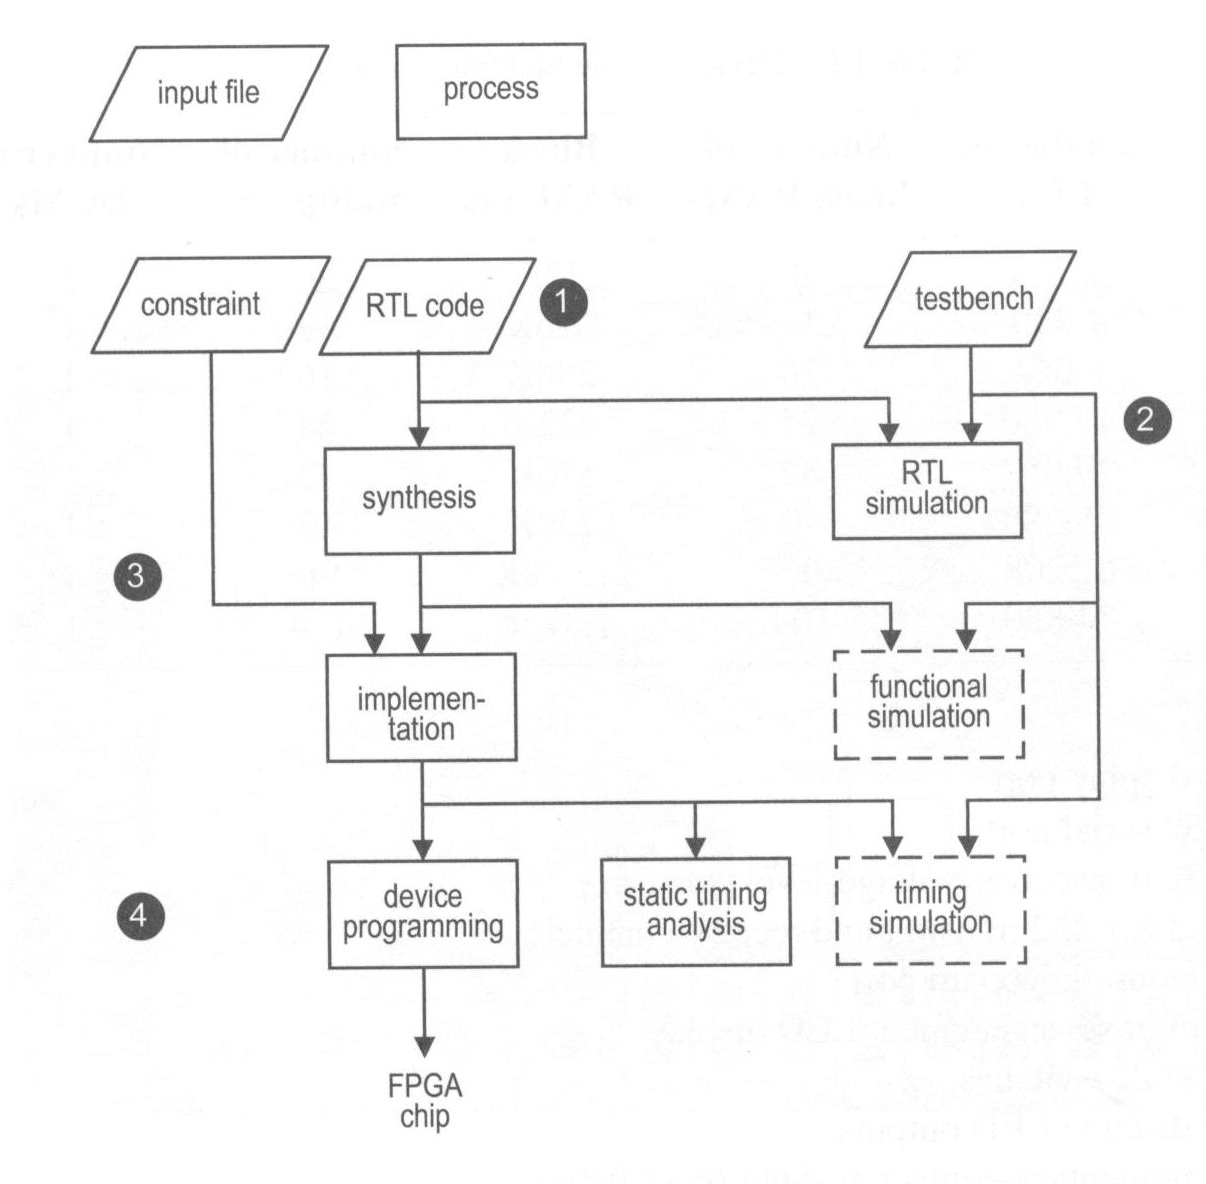
\includegraphics[width=0.5\textwidth]{pics/designprocess}
\end{center}

\subsection{Prozesse}
	\begin{itemize}
		\setlength{\itemsep}{1pt}
  	\setlength{\parskip}{0pt}
  	\setlength{\parsep}{0pt}
		\item Prozesse werden durch �nderungen an den Signalen in der Sensitivit�tsliste (im Prozess-Kopf) aktiviert und ausgef�hrt.
		\item Prozesse werden parallel abgearbeitet
		\item Innerhalb des Prozesses werden Anweisungen sequentiell abgearbeitet
		\item Selektive und konditionale Signalzuweisungen sind verboten.
		\item Unbedingte Signalzuweisung erlaubt. Aktualisierung aller Signale geschieht immer erst am Prozessende!
		\item G�ltig ist letzte Zuweisung
	\end{itemize}
	
	\lstinputlisting[language=vhdl,tabsize=2]{code/process.vhd}

\subsection{VHDL Code Example}
	\begin{center}
		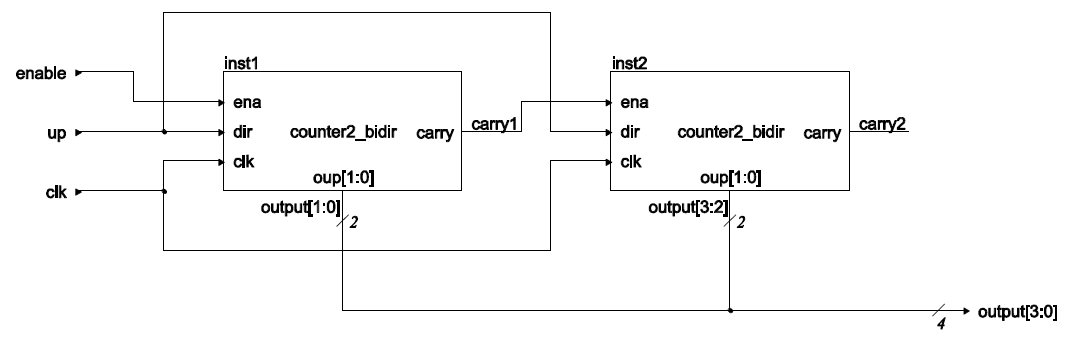
\includegraphics[width=0.5\textwidth]{pics/vhdlcodeexampleschematic.png}
	\end{center}
	\begin{multicols}{2}
		\lstinputlisting[language=vhdl,tabsize=2]{code/vhdlcodeexample.vhd}
	\end{multicols}		
%\section{Realisierungs Methoden}
\subsection{ROM}
Mit einem ROM lassen sich sich kombinatorische Schaltungen in Form einer Look up Table realisieren.\\
\begin{itemize}
	\setlength{\itemsep}{1pt}
  \setlength{\parskip}{0pt}
  \setlength{\parsep}{0pt}
  
	\item Eingangsvariablen = Adresse\\
	\item Speicherwert = Ausgang (programmierbar)\\
\end{itemize}

\begin{itemize}
	\setlength{\itemsep}{1pt}
  \setlength{\parskip}{0pt}
  \setlength{\parsep}{0pt}
  
	\item ROM $\rightarrow$ Bei der Herstellung programmierter Speicher\\
	\item PROM $\rightarrow$ Programmierbares ROM (Fuses)\\
	\item EPROM $\rightarrow$ L"oschbares PROM (UV Licht)\\
	\item EEPROM $\rightarrow$ Elektrisch l"oschbares PROM\\
	\item Flash $\rightarrow$ Blockweise beschreibbares EEPROM (schneller)\\
\end{itemize}

\subsection{PLD}
Programmierbares Device aus AND und OR-Matrix, mindestens eine Matrix programmierbar.
\begin{itemize}
	\setlength{\itemsep}{1pt}
  \setlength{\parskip}{0pt}
  \setlength{\parsep}{0pt}
  
	\item PAL $\rightarrow$ OR-Matrix fest, AND-Matrix programmierbar, Fuses\\
	\item PLA $\rightarrow$ OR und AND Matrix frei programmierbar, Fuses\\
	\item GAL $\rightarrow$ Wie PLA plus programmierbare Ausgangsnetzwerke (Tristate), EEPROM\\
\end{itemize}
F�r Funktionen die als DNF vorliegen geeignet, heute gr�sstenteils von CPLD und FPGA verdr�ngt.\\

\subsection{CPLD}
\begin{itemize}
	\setlength{\itemsep}{1pt}
  \setlength{\parskip}{0pt}
  \setlength{\parsep}{0pt}
  
	\item Verbund PLD Makrozellen die mit Bussen verbunden sind, Speicherung der Konfiguration in Flash.\\
	\item	Durch regelm"assige Struktur sind Signallaufzeiten vorhersagbar.\\
	\item Wegen grosser Zahl an Logikbl�cken sehr gut f�r parallele Prozesse geeignet.\\
\end{itemize}

\subsection{FPGA}
2D-Array von Logikbl"ocken, die �ber Routing Kanal und Schaltmatrizen miteinander und mit I/O verbunden werden.\\
\begin{itemize}
	\setlength{\itemsep}{1pt}
  \setlength{\parskip}{0pt}
  \setlength{\parsep}{0pt}
  
	\item Logikblock (LogicCell) $\rightarrow$ Lookuptable mit D-FlipFlop, kann beliebige Funktionen ausf"uhren
	\item Schaltmatrizen $\rightarrow$ programmierbare Verbindungen
	\item Makrozellen $\rightarrow$ Feste Funktionen z.B. Memory, Clock Managment...
\end{itemize}
Die Konfiguration wird im RAM gespeichert (fl"uchtig). D.h. bei jedem Boot muss der Code von einem Festspeicher geladen werden.\\

\subsection{Xilinx Spartan 3}
\begin{itemize}
	\setlength{\itemsep}{1pt}
  \setlength{\parskip}{0pt}
  \setlength{\parsep}{0pt}

	\item Logic Cell (LC): Kleinste Einheit, enth"alt LUT mit 4 Eing"angen und eime D-FlipFlop. LUT kann als 16x1 bit SRAM oder Schieberegister 		konfiguriert werden. Zus"atzlich pro LC CarryLogic und MUX.
	\item Slice: 1Slice = 2 Logic Cell
	\item Configurable logic bloc (CLB): 1 CLB = 4 Slices = 8 Locic Cells. \\
	Inerhalb dieser Einheit existieren spezifische Verbindungsstrukturen.
\end{itemize}

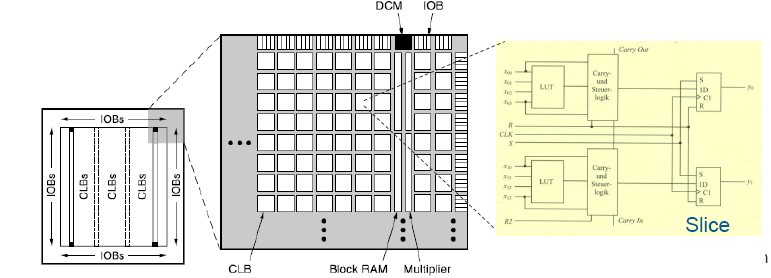
\includegraphics[width=0.8\textwidth]{pics/fpgastruct}


\subsection{Semicustom IC}
\begin{itemize}
	\setlength{\itemsep}{1pt}
  \setlength{\parskip}{0pt}
  \setlength{\parsep}{0pt}
  
	\item Mikrozellen aus p- und n-FETs werden durch Verdrahtung zu Gates.\\
	\item Gates k"onnen durch Verdrahtungskan"ale verbunden werden.\\
	\item Standardfunktionen k"onnen mit IP-Cores implementiert werden.\\
\end{itemize}	
	
\subsection{Fullcustom IC}
V�llig kundenspezifische ICs, oft werden IP-Cores f�r Standardfunktionen verwendet. Digitale und analoge Komponenten auf einem IC m�glich. Voll auf Anwendung anpassbare Eigenschaften (Stromverbrauch, Gr"osse, Geschwindigkeit etc.).\\

\subsection{Vergeichstabelle}

\begin{center}
	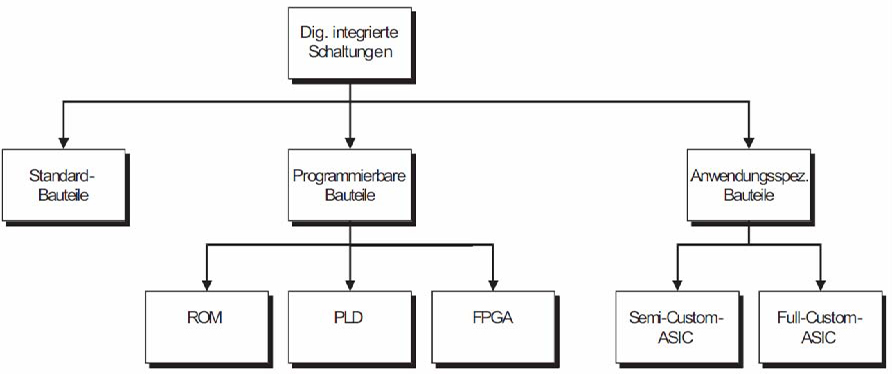
\includegraphics[width=0.60\textwidth]{pics/devicecomparetables}
	
	\begin{tabular}{|l|c|c|c|c|c|c|}
		\hline
		Kriterien & Standard Bauteile & ROM & PLD & FPGA & Semicustom & Fullcustom \\
		\hline
		Machbarkeit & ++ & - - & - - & + & + & +++ \\
		\hline
		Zeit Realisiertung & + & ++ & ++ & ++ & - & - - \\
		\hline
		Iterationszeit & - & ++ & ++ & ++ & - & - - \\
		\hline
		NRE & ++ & + & + & + & - & - - -\\
		\hline
		St"uckpreis & - - & + & + & - & + & +++ \\
		\hline
	\end{tabular}
\end{center}
	
\section{Logische Gatter}

	\subsection{Verhalten logischer Gatter}
		\begin{multicols}{2}
			\subsubsection{St"orabstand}
				High-Pegel: $ U_{n_H} = U_{a_Hmin} - U_{e_Hmin} $\\
				Low-Pegel: $ U_{n_L} = U_{e_Lmax} - U_{a_Lmax} $\\
				
		%\end{multicols}

		%\begin{multicols}{2}
			\subsubsection{Propagation delay (Verz"ogerungszeit) }
				Zeit zwischen 50\% von $V_{max}$ am Eingang und 50\% von $V_{max}$ am Ausgang.\\
				$t_{pd}=\frac{t_{p_{LH}}+t_{p_{HL}}}{2}$\\
				
			\subsubsection{Transition time (Übergangszeit)}
				Zeit zwischen 10\% und 90\% von $V_{max}$.\\
				$t_{t_{LH}}$: Transition time low to high.\\
				$t_{t_{HL}}$: Transition time high to low.\\
				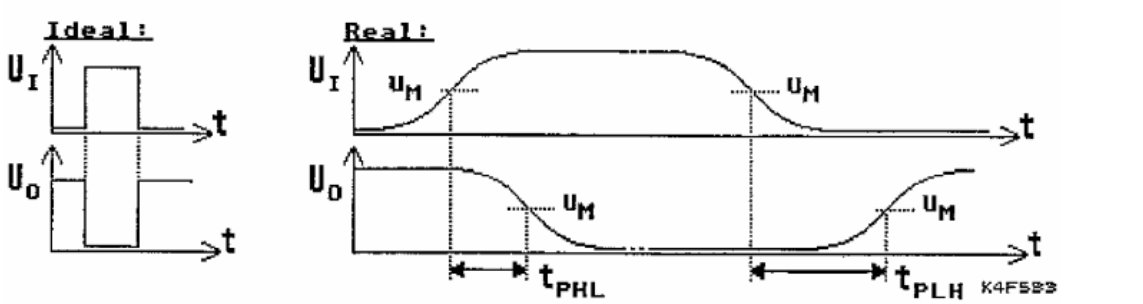
\includegraphics[width=0.2\textwidth]{pics/delay}
				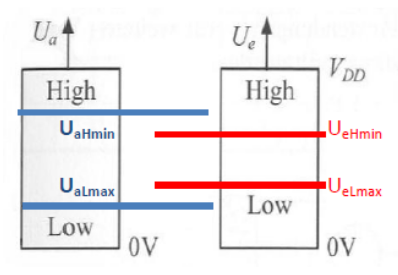
\includegraphics[width=0.2\textwidth]{pics/Pegelbereiche_Stoerabstand}
		\end{multicols}

\subsection{Hazards}
\begin{tabular}{rp{5cm}p{1cm}rp{5cm}}
	\textbf{statisch:}&kurzzeitige Änderung, obwohl keine Änderung gegeben ist.&&
	\textbf{dynamisch:}&mehrere Änderungen, obwohl nur eine Änderung gegeben ist.\\
\end{tabular}\\
\textbf{Vermeiden von Hazards:} Redundante Schaltungselemente einfügen (Fielen bei KV-Diagramm weg)
		


%\newpage
\begin{sidewaystable}
\subsection{Aufbau logischer Gatter}
\begin{tabular}{|c|c|c|c|c|c|c|c|c|}
\hline
Funktion & Buffer & NOT & AND & NAND & OR & NOR & EXOR & XNOR\\
& & Nicht & Und & Nicht Und & Oder & Nicht Oder & Exklusiv Oder & Nicht Ex. Oder\\
& & Inverter & Konjunktion & & Disjunktion & & Antivalenz & "Aquivalenz \\
\hline
Formel & a & $ \overline a $ & $ a \cdot b $ & $ \overline{a \cdot b} $ & $ a + b $ & $ \overline{a + b} $ & $ a \oplus b $ & $ \overline{a \oplus b} $\\
& a & $ \overline a $ & $ a \wedge b $ & $ \overline{a \wedge b} $ & $ a \vee b $ & $ \overline{a \vee b} $ & $ a \not= b $ & $ \overline{a \not= b} $ \\
& a & !a & $ a \& b $ & $ !(a \& b) $ & a\#b & !(a\#b) & a\$b & !(a\$b) \\
\hline
& & & & & & & &\\
& 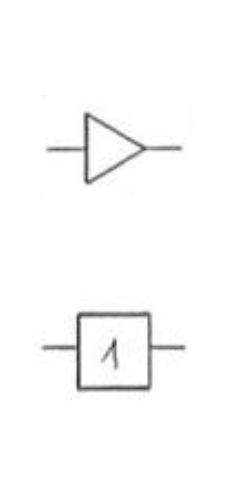
\includegraphics[width=0.08\textwidth]{pics/gates_symbol/buffer} & 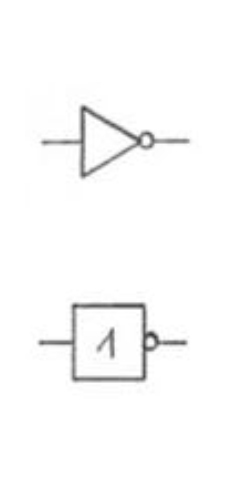
\includegraphics[width=0.08\textwidth]{pics/gates_symbol/not} & 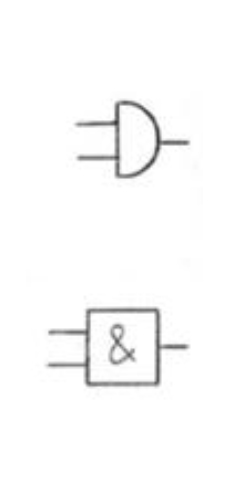
\includegraphics[width=0.08\textwidth]{pics/gates_symbol/and} & 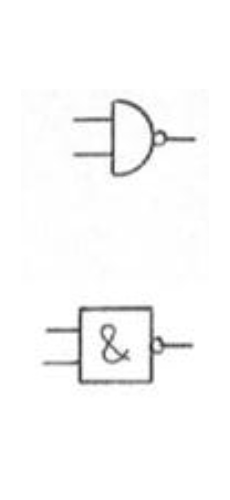
\includegraphics[width=0.08\textwidth]{pics/gates_symbol/nand} & 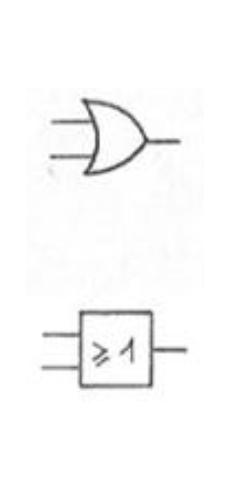
\includegraphics[width=0.08\textwidth]{pics/gates_symbol/or} & 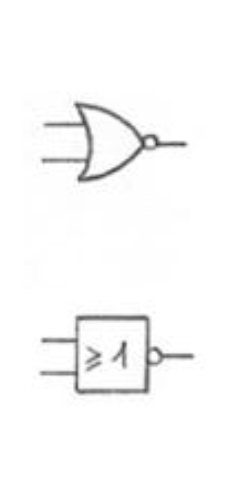
\includegraphics[width=0.08\textwidth]{pics/gates_symbol/nor} & 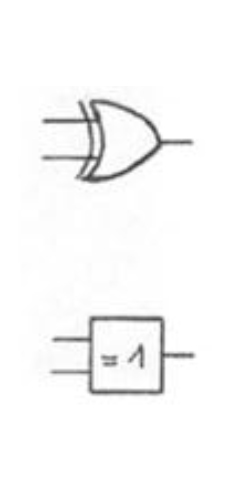
\includegraphics[width=0.08\textwidth]{pics/gates_symbol/exor} & 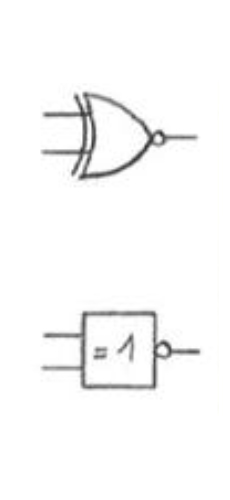
\includegraphics[width=0.08\textwidth]{pics/gates_symbol/xnor} \\
\hline
(0,0) & 0 & 1 & 0 & 1 & 0 & 1 & 0 & 1\\
(0,1) &   &   & 0 & 1 & 1 & 0 & 1 & 0\\
(1,0) & 1 & 0 & 0 & 1 & 1 & 0 & 1 & 0\\
(1,1) &   &   & 1 & 0 & 1 & 0 & 0 & 1\\
\hline
KDNF & \#(1) & \#(0) & \#(3) & \#(0,1,2) & \#(1,2,3) & \#(0) & \#(1,2) & \#(0,3) \\
KKNF & \&(0) & \&(1) & \&(0,1,2) & \&(3) & \&(0) & \&(1,2,3) & \&(0,3) & \&(1,2)\\
\hline
& & & & & & & &\\
& & 
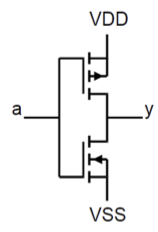
\includegraphics[width=0.12\textwidth]{pics/gates_schematic/inverter} & 
$ \overline{NAND} $ &
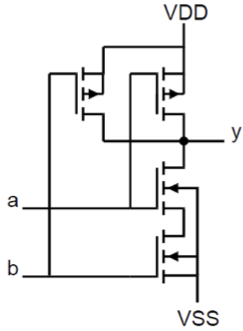
\includegraphics[width=0.12\textwidth]{pics/gates_schematic/NAND} &
$ \overline{NOR} $ &
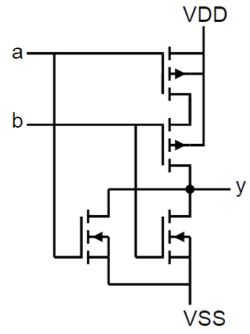
\includegraphics[width=0.12\textwidth]{pics/gates_schematic/NOR} & 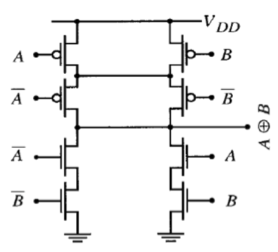
\includegraphics[width=0.12\textwidth]{pics/gates_schematic/XOR} & 
\\
\hline
\#Trans & & 2 & 6 & 4 & 6 & 4 & 8 & \\
\hline
\end{tabular}
\end{sidewaystable}
\section{Sequentielle Systeme}

\subsection{Taktsignal}
	\begin{minipage}{8 cm}
		Weil sequentielle Schaltungen in der Regel synchron arbeiten, muss eine Referenz zur Einhaltung der Synchronit"at definiert werden. Das Taktsignal ist ein bin"are Signal, das in regelm"assiger Abfolge zwischen zwei Zust"anden hin und her pendelt.
	\end{minipage}
	\begin{minipage}{0.5 cm}
		\ 
	\end{minipage}
	\begin{minipage}{7 cm}
		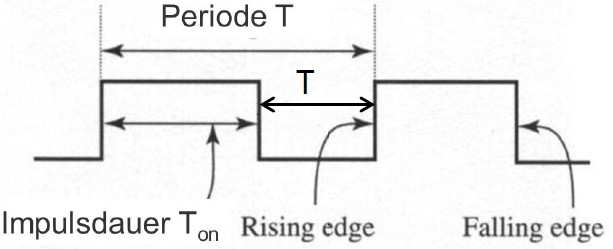
\includegraphics[width=0.9\textwidth]{pics/taktsignal}
	\end{minipage}
	\begin{minipage}{2 cm}
		$f=\frac{1}{T}$ [Hz]
	\end{minipage}

\subsection{Flipflops und Latches}
	\subsubsection{Unterschied Flipflop und Latch}
		\begin{minipage}{12 cm}
			Taktzustandsgesteuerte Systeme haben den Nachteil, dass in ihrer transparenten Phase auch asynchrone Schaltvorg"ange stattfinden k"onnen. Echt synchrone Systeme "andern ihren Zustand nur bei der aktiven Flanke des Taktsignals. Genau in diesem Moment und sonst nie wird das Eingangssignal bei einem Speicherelement in den Speicher "ubertragen. Nur beim taktflankengesteuerten System wechseln die Ausg"ange immer genau zum Zeitpunkt der aktiven Taktflanke. Beim taktzustandsgesteuerten System sind w"ahrend der transparenten Phase auch Zustands"anderungen zwischen zwei Taktflanken m"oglich. \\
			Taktflankengesteuerte Speicherelemente werden Flip-Flops genannt. Taktzustandsgesteuerte Speicherelemente werden Latches genannt
		\end{minipage}
		\begin{minipage}{0.5 cm}
			\ 
		\end{minipage}
		\begin{minipage}{6 cm}
			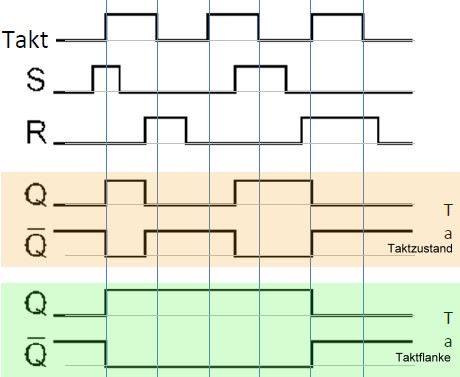
\includegraphics[width=0.9\textwidth]{pics/flipflop_latch}
		\end{minipage}
		
	\subsubsection{Transmission Gate}
		\begin{minipage}{10 cm}
			Das Transmission Gate ist von seiner Funktion her ein einfacher Schalter, der Signale sowohl auf positivem, als auch auf negativem Pegel schalten kann.
		\end{minipage}
		\begin{minipage}{0.5 cm}
			\ 
		\end{minipage}
		\begin{minipage}{8 cm}
			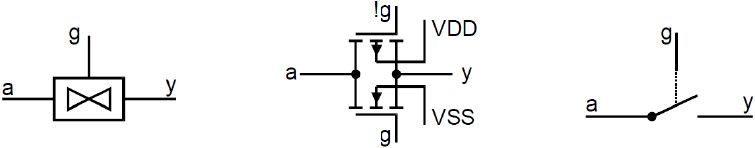
\includegraphics[width=0.9\textwidth]{pics/transmissiongate}
		\end{minipage}
		
	\begin{multicols}{2}
		\subsubsection{RS-Latch}
			\begin{minipage}{4 cm}
				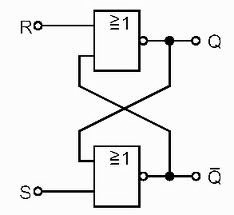
\includegraphics[width=0.9\textwidth]{pics/rs_latch}
			\end{minipage}
			\begin{minipage}{4 cm}
				\begin{tabular}{|cc|cc|}
					\hline
						S & R & $Q$ & $\overline{Q}$ \\
					\hline	
						0 & 0 & $Q$ & $\overline{Q}$ \\
						0 & 1 & 0 & 1 \\
						1 & 0 & 1 & 0 \\
						1 & 1 & \multicolumn{2}{c|}{ung"ultig} \\
					\hline
				\end{tabular}
			\end{minipage}
		
		\subsubsection{RS-Latch mit Clock}
			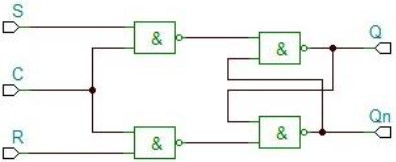
\includegraphics[width=0.4\textwidth]{pics/rs_latch_clock}
		\columnbreak
		
		\subsubsection{D-Latch}
			\begin{minipage}{4 cm}
				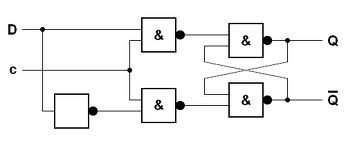
\includegraphics[width=0.9\textwidth]{pics/dlatch}
			\end{minipage}
			\begin{minipage}{4 cm}
				\begin{tabular}{|cc|cc|}
					\hline
						D & C & $Q$ & $\overline{Q}$ \\
					\hline	
						0 & 0 & $Q$ & $\overline{Q}$ \\
						0 & 1 & 0 & 1 \\
						1 & 0 & $Q$ & $\overline{Q}$ \\
						1 & 1 & 0 & 1 \\
					\hline
				\end{tabular}
			\end{minipage}
			
		\subsubsection{D-Flipflop mit Reset}
			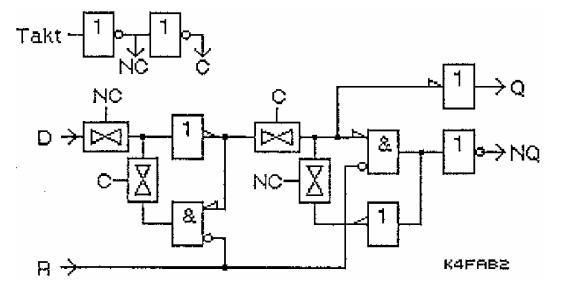
\includegraphics[width=0.4\textwidth]{pics/dflipflop}
	\end{multicols}
	
	\subsubsection{Setup- und Holdtime}
		\begin{minipage}{10 cm}
			\begin{compactitem}
				\item $t_s$= setup time $\rightarrow$ Minimale Zeitspanne, w"ahrend der ein Datensignal vor einer aktiven Clockflanke stabil sein muss, um zuverl"assig eingelesen zu werden.
				\item $t_H$= hold time $\rightarrow$ Minimale Zeitspanne, w"ahrend der ein Datensignal nach einer aktiven Clockflanke noch stabil bleiben muss, damit der Einlesevorgang des Datensignals erfolgreich abgeschlossen werden kann.
			\end{compactitem}
		\end{minipage}
		\begin{minipage}{0.5 cm}
			\ 
		\end{minipage}
		\begin{minipage}{8 cm}
			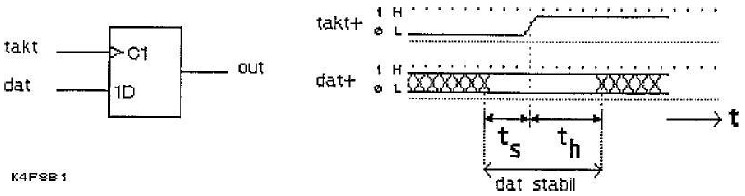
\includegraphics[width=0.9\textwidth]{pics/setupholdtime}
		\end{minipage}
		
\subsection{Beschreibung sequentieller Systeme}
	\begin{multicols}{2}
		\begin{compactitem}
			\item S: Menge der Zust"ande mit Zustandsaktionen
			\item I$\subseteq$S: Initalzust"ande
			\item T: Kombinatorische "Ubergangsrelation
			\item E: Eingangssignale
			\item A: Ausgangssignale
		\end{compactitem}
	\end{multicols}
	
	\begin{multicols}{2}
		\subsubsection{Tabellarische Beschreibung}
			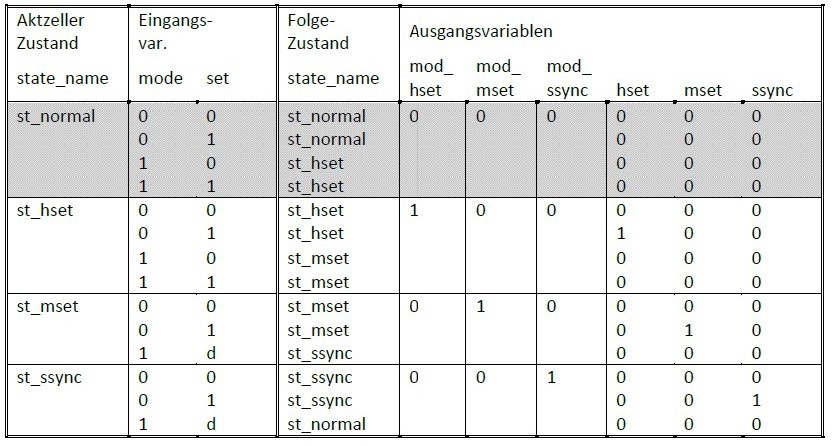
\includegraphics[width=0.49\textwidth]{pics/zustandstabelle}
		\columnbreak
		
		\subsubsection{Grafische Beschreibung (Zustandsdiagramm)}
			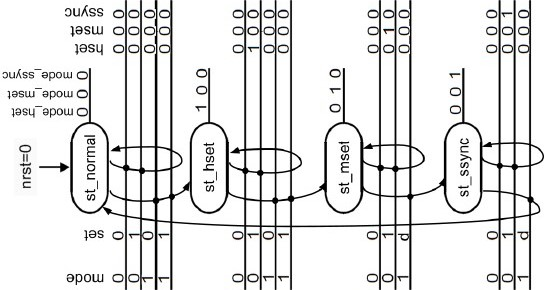
\includegraphics[width=0.5\textwidth]{pics/zustandsdiagramm}
	\end{multicols}
	Diese Beispiele visualisieren das sequentielle System des Watch-Controllers.
	
\subsection{Strukturen der Finite State Machine}
	\begin{multicols}{3}
		\subsubsection{Grundstruktur}
			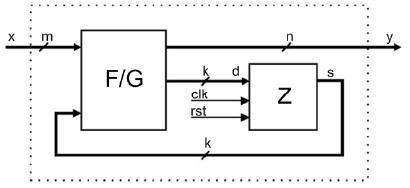
\includegraphics[width=0.3\textwidth]{pics/seq_grundstruktur}
		\columnbreak
		
			\begin{compactitem}
				\item s: Zustand, Zustandsvektor
				\item x: Prim"are Eing"ange, Eingangsvektor
				\item y: Prim"are Ausg"ange, Ausgangsvektor
				\item d: Speicheransteuerung, Folgezustand
				\item m: Anzahl Eing"ange
				\item n: Anzahl Ausg"ange
				\item k: Anzahl Speicherstellen
				\item F: Funktion f"ur die Ausg"ange
				\item G: Funktion f"ur die Speicheransteuerung
				\item Z: Zustandsspeicher
				\item I: Index der aktuellen Taktflanke (Taktflankennummer)
			\end{compactitem}
	\end{multicols}
	
	\begin{multicols}{3}
		\subsubsection{Mealy-System}
			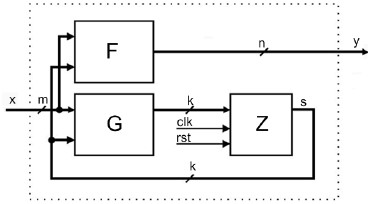
\includegraphics[width=0.26\textwidth]{pics/seq_mealy}
			Ausg"ange h"angen vom momentanen Zustand und den aktuellen Eing"angen ab
			
		\subsubsection{Moore-System}
			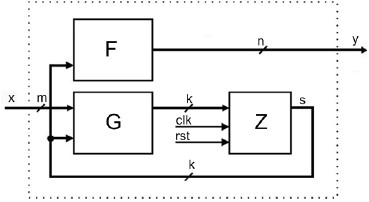
\includegraphics[width=0.26\textwidth]{pics/seq_moore}
			Ausg"ange h"angen nur vom momentanen Zustand ab und "andern mit der Clock Flanke
			
		\subsubsection{Medwedjew-System}
			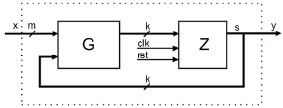
\includegraphics[width=0.3\textwidth]{pics/seq_medmedjew}
			Die prim"aren Ausg"ange entsprechen dem Zustandsvektor
	\end{multicols}
	
\subsection{Zustandscodierung}
	\begin{multicols}{3}
		\begin{compactitem}
			\item Bin"ar: Alle Zust"ande werden der Reihe nach durchnummeriert.
			\newline
			\newline
			\item ONE-HOT: Nur eine Speicherstelle im Code hat jeweils den Wert 1. Alle anderen besitzen den Wert 0 (z.B. 001, 010, 100)
			\item ONE-COLD: Nur eine Speicherstelle im Code hat jeweils den Wert 0. Alle anderen besitzen den Wert 1 (z.B. 110, 101, 011)
		\end{compactitem}
	\end{multicols}
	
\subsection{Synthese von Zustandsmaschinen}
	\begin{multicols}{2}
		\begin{enumerate}
			\setlength{\itemsep}{1pt}
			\setlength{\parskip}{0pt}
			\setlength{\parsep}{0pt}
			\item Zustandsdiagramm aufstellen
			\item Zustandskodierung zuweisen
			\item Zustandstabelle nach festen Regeln aufstellen
			\item Speicheransteuer-Funktionen bestimmen
			\item Ausgangs-Funktionen bestimmen
		\end{enumerate}
	\end{multicols}

\end{document}
